\section{Interface Class Diagram}
In questa sezione si definiscono in alto livello le interfacce, con relativi metodi, per la comunicazione tra i componenti e sottosistemi ottenuti. In particolare, vengono definiti con lo stereotipo \textbf{signal} i canali di comunicazione ad eventi, designati nel progetto per seguire un pattern publisher-subscriber.

\subsection{Interfacce Gestione Comanda}
\begin{figure}[H]
	\centering
	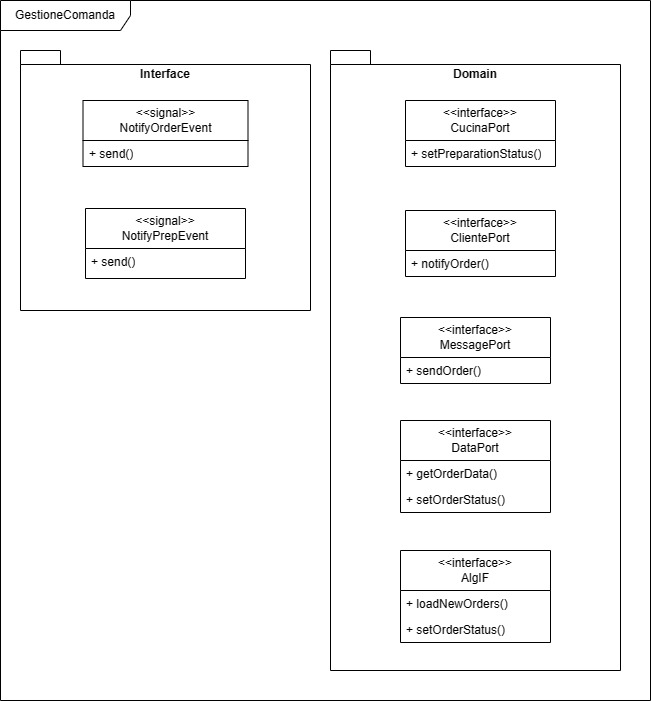
\includegraphics[scale=0.5]{iterazione1/images/GestioneComanda interface UML.jpg}
	\caption{Interface class diagram - Gestione Comanda\label{fig:interface_class_diagram_gestione_comanda}}
\end{figure}

\subsection{Interfacce Gestione Cucina}
\begin{figure}[H]
	\centering
	\includegraphics[scale=0.5]{iterazione1/images/GestioneCucina interface UML.jpg}
	\caption{Interface class diagram - Gestione Cucina\label{fig:interface_class_diagram_gestione_cucina}}
\end{figure}

\subsection{Interfacce Gestione Cliente}
\begin{figure}[H]
	\centering
	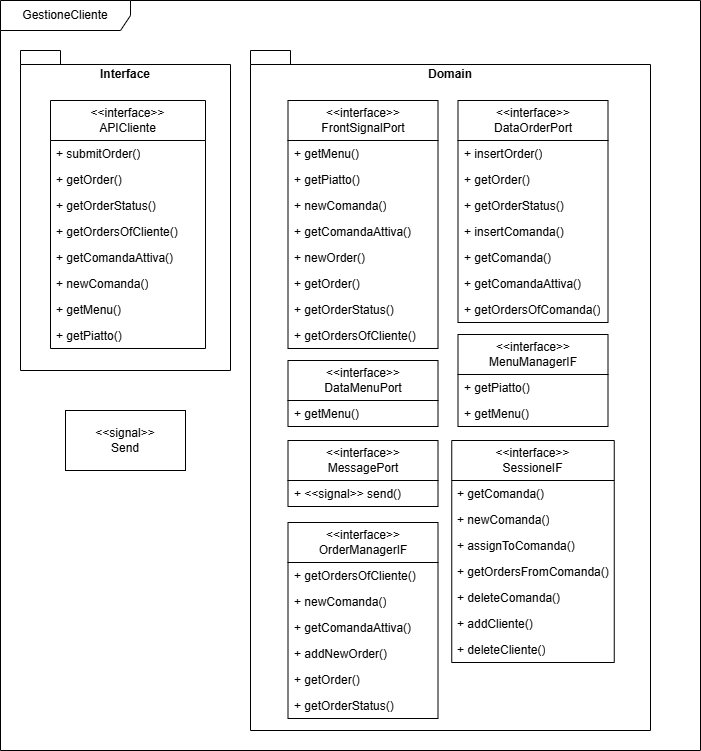
\includegraphics[scale=0.5]{iterazione1/images/GestioneCliente interface UML.jpg}
	\caption{Interface class diagram - Gestione Cliente\label{fig:interface_class_diagram_gestione_cliente}}
\end{figure}

\clearpage